\documentclass{article}
\usepackage{graphicx}
\usepackage{amsmath}
\usepackage[sorting=none]{biblatex}
\addbibresource{manual.bib}

\title{LIFTLINE Manual}
\author{Christopher C. Chinske}

\begin{document}
\maketitle
\newpage
\section{Introduction}
LIFTLINE is a collection of MATLAB scripts and functions that
implement lifting-line theory.  It solves the monoplane equation to
estimate aerodynamic characteristics of a finite wing.  It also
provides capabilities to analyze shear force and bending moment along
the wing spar.
\subsection{Theory}
LIFTLINE implements lifting-line theory as described in \cite{bertin}
and \cite{anderson}.  The program estimates the spanwise circulation
of a finite wing.  Following from this result, the program can compute
the lift and vortex-induced drag coefficients.  The program can also
estimate structural characteristics, such as shear and bending moment
along the wing.
\paragraph{}
Classical lifting-line theory assumes incompressible flow, no wing
sweep, and linear airfoil section lift-curve slopes.  Currently,
LIFTLINE assumes:
\begin{enumerate}
\item Incompressible flow
\item No wing sweep (input required to properly draw planform)
\item Linear airfoil section lift-curve slopes
\item Symmetrical loading.
\end{enumerate}
Future versions of LIFTLINE will implement a modified lifting-line
theory and relax these assumptions.
\subsection{Graphical Workflow}
\fbox{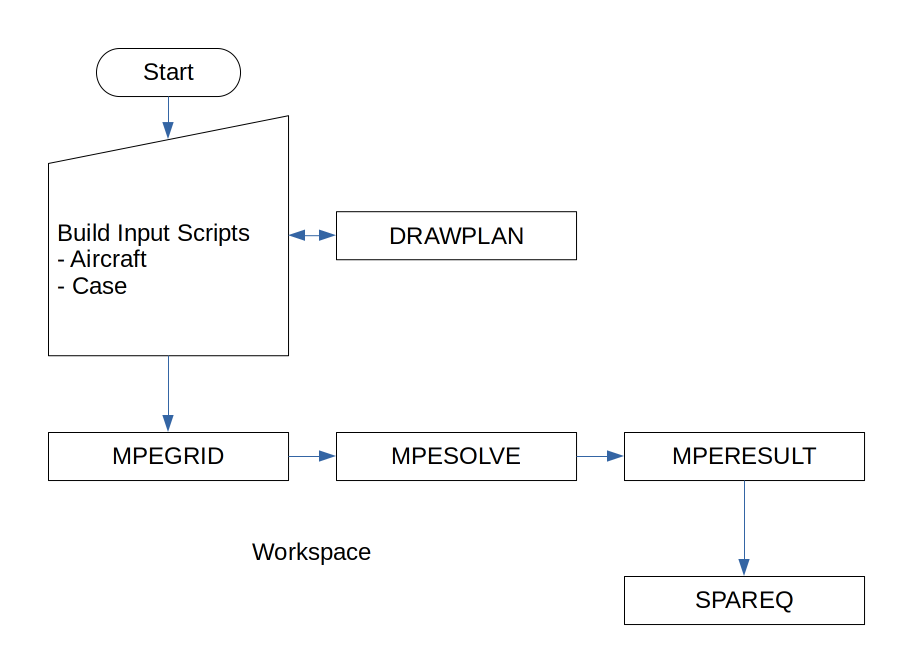
\includegraphics[width=\textwidth]{images/flowchart.png}}
\subsection{LIFTLINEUI}
The function LIFTLINEUI provides an interactive interface that guides
the user through common analyses.  These analyses are described below.
\begin{enumerate}
  \item Grid Convergence Analysis.  Find the number of Fourier sine
    series coefficients required to meet specified error requirements.
  \item Find AoA for L = W.  Find the angle of attack that generates
    lift equal to the weight of the aircraft specified in the
    aircraft script.
  \item Run Case.  Run MPEGRID, MPESOLVE, and MPERESULT using a
    specified case script.
  \item AoA Range.  Find CL and CDv over a range of angle of
    attack.
  \item Spar Shear and Bending Moment.  Compute and plot shear and
    bending moment along the wing.
\end{enumerate}
When building a new aircraft script, it's generally recommended to run
a grid convergence analysis at a small, positive angle of attack
(e.g., 4 deg).  Update the case script as necessary.  Then, if
considering an aircraft in steady flight, find the angle of attack for
L = W.  Again, update the case script as necessary.
\section{Definition of Inputs and Outputs}
\subsection{Basic Configuration Geometry Inputs}
N panels compose the semi-span.  For each row of clalp, alpzl, and
clmax, the inboard value applies immediately outboard of the panel's
inboard breakpoint.\\*\\*
\begin{tabular}{|l|l|p{2.5in}|c|}
  % --------------------------------------------------
  \hline
  \textbf{Variable Name} &
  \textbf{Dimension} &
  \textbf{Description} &
  \textbf{Units}
  \\
  \hline
  % --------------------------------------------------
%  var & dim &
%  description &
%  unit
%  \\
%  \hline
%  % --------------------------------------------------
  ybp & 1 x (N+1) &
  Spanwise coordinates of breakpoints [$0$, $y_1$, $y_2$, ..., $b/2$] &
  m
  \\
  \hline
  % --------------------------------------------------
  cbp & 1 x (N+1) &
  Chord at breakpoints [$c_r$, $c_1$, $c_2$, ..., $c_t$] &
  m
  \\
  \hline
  % --------------------------------------------------
  sweepa & 1 x N &
  Sweep angle (c/4) of each panel &
  deg
  \\
  \hline
  % --------------------------------------------------
  twista & 1 x N &
  Twist angle at tip of each panel &
  deg
  \\
  \hline
  % --------------------------------------------------
  clalp & N x 2 &
  Airfoil section lift-curve slope, $C_{l_\alpha}$.  Each row
  corresponds to a panel.  Column 1 is the inboard value.  Column 2 is
  the outboard value. &
  1/deg
  \\
  \hline
  % --------------------------------------------------
  alpzl & N x 2 &
  Airfoil section zero lift angle of attack, $\alpha_{0l}$.  Each row
  corresponds to a panel.  Column 1 is the inboard value.  Column 2 is
  the outboard value. &
  deg
  \\
  \hline
  % --------------------------------------------------
  clmax & N x 2 &
  Airfoil section maximum lift coefficient, $C_{l_{max}}$.  Each row
  corresponds to a panel.  Column 1 is the inboard value.  Column 2 is
  the outboard value. &
  -
  \\
  \hline
  % --------------------------------------------------
  b & Scalar &
  Span &
  m
  \\
  \hline
  % --------------------------------------------------
  S & Scalar &
  Reference wing area &
  m\^{}2
  \\
  \hline
  % --------------------------------------------------
  W & Scalar &
  Weight &
  N
  \\
  \hline
  % --------------------------------------------------
\end{tabular}
\subsection{MPEGRID, MPESOLVE, and MPERESULT}
In addition to subsets of the basic configuration geometry inputs, the
functions MPEGRID, MPESOLVE, and MPERESULT use inputs/outputs as
defined below.  N is the number of Fourier sine series
coefficients.\\*\\*
\begin{tabular}{|l|l|p{2.5in}|c|}
  % --------------------------------------------------
  \hline
  \textbf{Variable Name} &
  \textbf{Dimension} &
  \textbf{Description} &
  \textbf{Units}
  \\
  \hline
  % --------------------------------------------------
  alpha\_r & Scalar &
  Angle of attack (root) &
  deg
  \\
  \hline
  % --------------------------------------------------
  ncoef & Scalar &
  Number of Fourier sine series coefficients &
  -
  \\
  \hline
  % --------------------------------------------------
  theta & 1 x N &
  Transformed spanwise coordinate &
  rad
  \\
  \hline
  % --------------------------------------------------
  y & 1 x N &
  Spanwise coordinate &
  m
  \\
  \hline
  % --------------------------------------------------
  c & 1 x N &
  Chord &
  m
  \\
  \hline
  % --------------------------------------------------
  a0 & 1 x N &
  Section lift-curve slope &
  1/rad
  \\
  \hline
  % --------------------------------------------------
  alpha & 1 x N &
  Section angle of attack &
  rad
  \\
  \hline
  % --------------------------------------------------
  alpha\_zl & 1 x N &
  Section zero lift angle of attack &
  rad
  \\
  \hline
  % --------------------------------------------------
  clmax\_vec & 1 x N &
  Section maximum lift coefficient &
  -
  \\
  \hline
  % --------------------------------------------------
  An & 1 x N &
  Fourier coefficients [$A_1$, $A_3$, ..., $A_{2N-1}$] &
  -
  \\
  \hline
  % --------------------------------------------------
  U & Scalar &
  Free-stream velocity &
  m/s
  \\
  \hline
  % --------------------------------------------------
  Gamma & 1 x N &
  Circulation &
  m\^{}2/s
  \\
  \hline
  % --------------------------------------------------
  CL & Scalar &
  Wing lift coefficient &
  -
  \\
  \hline
  % --------------------------------------------------
  CDv & Scalar &
  Wing vortex-induced drag coefficient &
  -
  \\
  \hline
  % --------------------------------------------------
  cl & 1 x N &
  Section lift coefficient &
  -
  \\
  \hline
  % --------------------------------------------------  
\end{tabular}
\subsection{SPAREQ}
The function SPAREQ (Spar Equilibrium Shear and Bending Moment)
optionally uses the inputs ploads and uloads, as defined below.  Other
inputs/outputs are also defined below.\\*\\*
\begin{tabular}{|l|l|p{2.5in}|c|}
  % --------------------------------------------------
  \hline
  \textbf{Variable Name} &
  \textbf{Dimension} &
  \textbf{Description} &
  \textbf{Units}
  \\
  \hline
  % --------------------------------------------------
  ploads & R x 2 &
  Point loads applied along the wing.  Each row specifies a point
  load.  Column 1, y-values (meters).  Column 2, loads.  Negative
  loads values apply in the downward direction.  For example, a store
  would be input as a negative load.  Example:
  $\begin{bmatrix}1.2&-50\\2.1&-25\\\end{bmatrix}$ &
  N
  \\
  \hline
  % --------------------------------------------------
  uloads & R x 3 &
  Uniform distributed loads applied along the wing.  Column 1, inboard
  y-values (meters).  Column 2, outboard y-values (meters).  Column 3,
  load per unit span.  Negative loads values apply in the downward
  direction.  For example, a fuel tank would be input as a negative
  load.  Example:
  $\begin{bmatrix}1.1&2.2&-10\\2.0&4.0&-20\\\end{bmatrix}$ &
  N/m
  \\
  \hline
  % --------------------------------------------------
  rho & Scalar &
  Density &
  kg/m\^{}3
  \\
  \hline
  % --------------------------------------------------
  V & 1 X N &
  Shear &
  N
  \\
  \hline
  % --------------------------------------------------
  M & 1 X N &
  Bending Moment &
  N*m
  \\
  \hline
  % --------------------------------------------------
  M\_root & 1 X N &
  Root Bending Moment &
  N*m
  \\
  \hline
  % --------------------------------------------------  
\end{tabular}
\newpage
\printbibliography
\end{document}
